\documentclass[11pt,a4paper]{article}
\usepackage[margin=20mm]{geometry}
\usepackage[T1]{fontenc}
\usepackage{lmodern}
\usepackage{tabularx,booktabs,longtable,array}
\usepackage{hyperref}
\usepackage{xcolor}
\usepackage{enumitem}
\usepackage{graphicx}
\usepackage{float}
\usepackage{tikz}
\usetikzlibrary{arrows.meta,positioning}
\hypersetup{colorlinks=true,linkcolor=blue,urlcolor=blue,citecolor=blue}
\setlength{\parindent}{0pt}
\setlength{\parskip}{5pt}
\renewcommand{\arraystretch}{1.15}
\newcommand{\code}[1]{\texttt{#1}}
\newcommand{\imageplaceholder}[2]{\begin{figure}[H]\centering\fbox{\begin{minipage}[c][#1][c]{0.88\linewidth}\centering\Large IMAGE PLACEHOLDER\\[8pt]\normalsize #2\\[8pt]\small Replace this box with the corresponding diagram or screenshot.\end{minipage}}\caption{#2}\end{figure}}
\title{\textbf{23CSE455 Design Patterns}\\Case Study Report}
\date{28 October 2026}
\begin{document}
\maketitle
\begin{center}
\textbf{Case Study: Design Pattern Discovery and Evolution in the MBTA API}\\[4pt]
\textbf{Team: A2}
\end{center}
\textbf{Application:} MBTA API — \url{https://github.com/mbta/api}\\
\textbf{Submission repository:} \url{https://github.com/aswathymohan-amrita/23CSE455_DP_CaseStudy}\\
\textbf{Report date:} 2026-10-28

\textbf{Students}
\begin{tabularx}{\linewidth}{@{}lXl@{}}
\toprule Roll number & Student name & Batch\\ \midrule
AM.SC.U4CSE23201 & Aadhav Gugan DU & A\\
AM.SC.U4CSE23220 & G Yaswanth Ram Saran & A\\
AM.SC.U4CSE23227 & KB Sai Prasad Reddy & A\\
\bottomrule
\end{tabularx}


\tableofcontents
\newpage

% ============================================================
\section{Application and Architecture}
% ============================================================
\subsection{Application Overview}
The Massachusetts Bay Transportation Authority (MBTA) API is a service-oriented application that exposes transportation data and related operations through application endpoints. The source examined for this case study is the MBTA API repository. The study focuses on two selected collaborations that illustrate the Strategy design pattern: backend selection for rate limiting and parser selection for state data.

The case study has three parts. Part 1 identifies candidate design-pattern collaborations in the original source. Part 2 examines three changes prepared in a saved evolved source copy and records their observable test evidence and pattern effects. Part 3 builds small representative examples in Java, Python, JavaScript, and C++ to compare how the same broad Strategy idea can be expressed across languages. The Part 3 programs are educational examples, not direct ports of the complete Elixir application.

\subsection{Source and Environment}
\begin{tabularx}{\linewidth}{@{}p{0.27\linewidth}X@{}}
\toprule Item & Recorded information\\ \midrule
Repository & \url{https://github.com/mbta/api}\\
Source acquisition & A downloaded source archive was inspected. An exact baseline Git commit was not verified from the available extracted source.\\
Primary language/framework & Elixir and Phoenix, with application code organized into umbrella applications.\\
Required tool versions & The repository's \code{.tool-versions} specifies Elixir \code{1.19.5-otp-28} and Erlang/OTP \code{28.5.0.3}.\\
Local Part 3 JavaScript runtime & Node.js v24.15.0 was observed on the Windows host.\\
Local Part 3 C++ compiler & GCC 16.2.0 from MSYS2 UCRT64, using C++17, was observed.\\
Java and Python versions & Not recorded in the available test evidence.\\
License/dependencies & Exact license and a complete dependency-version manifest were not independently confirmed in the available materials.\\
\bottomrule
\end{tabularx}

The required Elixir/Erlang version information is reported from the repository version file, not as a claim that every local test was executed successfully under that toolchain. During setup, the machine initially had Erlang/OTP 29 installed, which did not match the repository's OTP 28 requirement. The Part 2 notes retain the distinction between targeted test evidence and the later compile warning encountered in the state application.

\subsection{Scope and Method}
The inspection scope was limited to the rate-limiter modules, parser modules, and state-server delegation paths relevant to the two selected collaborations. The principal paths were:
\begin{itemize}[leftmargin=*]
\item \code{apps/api\_web/lib/api\_web/rate\_limiter/} — rate limiter context, behaviour, and backend implementations.
\item \code{apps/parse/lib/parse.ex} and parser modules under \code{apps/parse/lib/parse/} — parser contract and implementations.
\item \code{apps/state/lib/state/server.ex} — state update handling and delegation to a configured parser.
\item Related tests under \code{apps/api\_web/test/} and \code{apps/state/test/} — observed verification evidence for the Part 2 changes.
\end{itemize}
Candidates were evaluated by tracing behaviour contracts, concrete modules, configuration values, callback implementations, and delegation calls. A module name or a pattern-like label was not considered sufficient by itself. The report describes the inspected scope and does not claim that the entire repository was exhaustively audited.

\subsection{Architecture}
The two selected collaborations use module-based polymorphism rather than requiring class inheritance. For rate limiting, the context reads the configured limiter implementation and delegates operations through a common behaviour. The ETS and Memcache modules are alternative backend implementations. For state parsing, the state server obtains a configured parser and delegates the relevant parse operation through the parser contract. Alerts, Line, and Routes are different parser implementations, with shared parsing support used where appropriate.

\begin{figure}[H]
\centering
\resizebox{0.97\linewidth}{!}{%
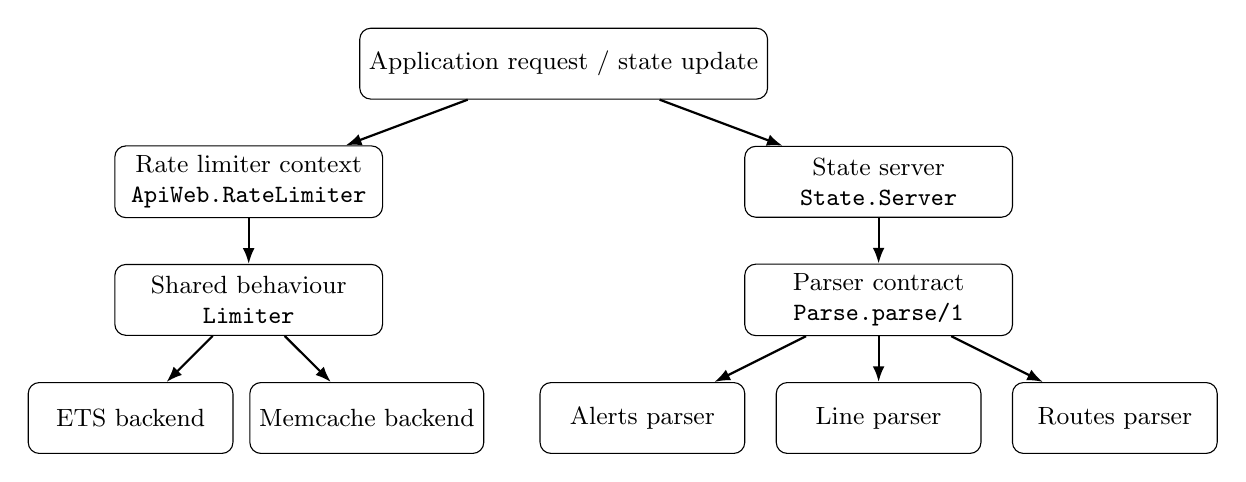
\begin{tikzpicture}[block/.style={draw,rounded corners,align=center,minimum width=34mm,minimum height=9mm,font=\small},leaf/.style={draw,rounded corners,align=center,minimum width=26mm,minimum height=9mm,font=\small},arr/.style={-{Latex[length=2mm]},thick}]
\node[block] (request) at (0,0) {Application request / state update};
\node[block] (rate) at (-4,-1.5) {Rate limiter context\\\code{ApiWeb.RateLimiter}};
\node[block] (server) at (4,-1.5) {State server\\\code{State.Server}};
\node[block] (limiter) at (-4,-3) {Shared behaviour\\\code{Limiter}};
\node[block] (parser) at (4,-3) {Parser contract\\\code{Parse.parse/1}};
\node[leaf] (ets) at (-5.5,-4.5) {ETS backend};
\node[leaf] (mem) at (-2.5,-4.5) {Memcache backend};
\node[leaf] (alerts) at (1,-4.5) {Alerts parser};
\node[leaf] (line) at (4,-4.5) {Line parser};
\node[leaf] (routes) at (7,-4.5) {Routes parser};
\draw[arr] (request) -- (rate); \draw[arr] (request) -- (server);
\draw[arr] (rate) -- (limiter); \draw[arr] (limiter) -- (ets); \draw[arr] (limiter) -- (mem);
\draw[arr] (server) -- (parser); \draw[arr] (parser) -- (alerts); \draw[arr] (parser) -- (line); \draw[arr] (parser) -- (routes);
\end{tikzpicture}%
}
\caption{Conceptual architecture of the two Strategy collaborations in the inspected scope.}
\label{fig:architecture}
\end{figure}

\subsection{Run Instructions and Test Evidence}
The original Elixir project should be run from the repository root using the repository's documented setup and version manager. The relevant test commands recorded for Part 2 are listed in Section 3. The Part 3 examples have separate test runners in each language directory; run each command from its corresponding folder. Commands and results in this report are based on recorded notes and user-reported local test outcomes. Summary evidence files should be checked against raw terminal output before final submission if the course requires raw logs.

% ============================================================
\section{Part 1: Pattern Discovery}
% ============================================================
\subsection{Discovery Method}
The discovery process began by identifying modules that expose a common contract and multiple alternative implementations. The candidate was then checked for an explicit context or delegator that selects an implementation and calls it through that contract. This approach helps distinguish a genuine Strategy collaboration from a set of unrelated modules that happen to perform similar work.

The analysis recorded the pattern name, category, meaningful instance name, participant roles, source paths, intent, and evidence. The two instances are treated as provisional confirmed Strategy collaborations within the inspected scope. Their classification is supported by behaviour/module contracts and delegation. A final audit should reconcile exact line ranges with the checked-out source and ensure that the CSV uses the required schema.

\subsection{Baseline Totals}
\begin{center}
\begin{tabularx}{0.92\linewidth}{@{}Xr@{}}
\toprule Measure & Count / status\\ \midrule
Distinct pattern types in the reported inventory & 1\\
Strategy candidate collaborations & 2\\
Rate Limiter Backend Selection & 1\\
State Data Parsing & 1\\
Concrete participant module total & Not consolidated\\
Unique participant-symbol total & Not consolidated\\
Rejected candidates & No reconciled total available\\
Uncertain candidates & No reconciled total available\\
\bottomrule
\end{tabularx}
\end{center}
The totals are limited to the two documented collaborations. Concrete participant totals are not guessed because a consistent counting convention has not been reconciled across the inventory. The same module may participate in multiple roles, and a shared parser-support module should not automatically be counted as an independent strategy instance.

\subsection{Pattern Inventory}
\begin{longtable}{@{}p{0.13\linewidth}p{0.30\linewidth}p{0.19\linewidth}p{0.30\linewidth}@{}}
\toprule Pattern & Instance name & Category & Main participants\\ \midrule
\endhead
Strategy & Rate Limiter Backend Selection & Behavioral / GoF & \code{ApiWeb.RateLimiter}, \code{ApiWeb.RateLimiter.Limiter}, ETS and Memcache backend modules.\\
Strategy & State Data Parsing & Behavioral / GoF & \code{State.Server}, \code{Parse.parse/1}, Alerts, Line, and Routes parser modules.\\
\bottomrule
\end{longtable}

\subsection{Instance 1: Rate Limiter Backend Selection}
\textbf{Pattern:} Strategy. \textbf{Category:} Behavioral GoF pattern. \textbf{Origin:} Application/framework implementation in the MBTA API source.

\textbf{Intent and problem addressed.} Rate-limiting behavior can be backed by different storage/limiting implementations. The application should be able to select a backend using configuration instead of embedding every backend-specific operation directly in the context. This separation allows the context to work against a common contract while backend modules supply the concrete behavior.

\textbf{Participant mapping.}
\begin{longtable}{@{}p{0.20\linewidth}p{0.36\linewidth}p{0.34\linewidth}@{}}
\toprule Strategy role & Actual symbol & Source location / evidence\\ \midrule
\endhead
Context / delegator & \code{ApiWeb.RateLimiter} & \code{apps/api\_web/lib/api\_web/rate\_limiter/}; reads configured limiter and delegates operations.\\
Strategy contract & \code{ApiWeb.RateLimiter.Limiter} & \code{limiter.ex}; declares the behaviour/callback contract.\\
Concrete strategy & \code{ApiWeb.RateLimiter.ETS} & Corresponding ETS backend module; implements the common behaviour.\\
Concrete strategy & \code{ApiWeb.RateLimiter.Memcache} & Corresponding Memcache backend module; alternative implementation under the same contract.\\
Configuration participant & Limiter configuration entry & Application configuration selects the implementation module.\\
\bottomrule
\end{longtable}

\textbf{Interaction and evidence.} The context obtains the configured limiter module and delegates operations such as \code{start\_link/1} and \code{rate\_limited?/2}. The alternative backends implement the same declared behaviour. The design therefore places the variation in the backend modules and lets the context invoke the chosen implementation through a shared contract. The evidence is the combination of behaviour declarations, callback implementations, configuration, and delegation calls; a backend class name alone would not establish Strategy.

\textbf{Why Strategy is appropriate.} The main variation point is the algorithm/backend used to answer a rate-limit query and manage its storage. The context does not need to know the concrete backend's internal representation to invoke the contract. This improves substitutability and isolates backend-specific concerns. The trade-off is that each backend must correctly honour the common contract and configuration must point to a compatible module.

\begin{figure}[H]
    \centering
    \includegraphics[width=0.70\linewidth,height=0.65\textheight,keepaspectratio]{rate_limiter_strategy.png}
    \caption{Strategy pattern for Rate Limiter Backend Selection in the MBTA API.}
    \label{fig:rate-limiter-strategy}
\end{figure}

\textbf{Verification and limitations.} The pattern claim is supported by source inspection in the scoped modules. Part 2 tests added coverage for rate limiter clearing, per-user independence, backend behavior, and concurrency. Those tests relate to the original Elixir application and should be kept distinct from the simplified cross-language rate limiter snippets, whose behavior is explicitly limited to delegation.

\subsection{Instance 2: State Data Parsing}
\textbf{Pattern:} Strategy. \textbf{Category:} Behavioral GoF pattern. \textbf{Origin:} Application-defined module selection and delegation.

\textbf{Intent and problem addressed.} The state server processes incoming state data that may need different parsing logic depending on the data type. Rather than making the server contain a large set of parser-specific branches, it delegates parsing to a configured parser module that implements the parser contract. This keeps the state update workflow separate from format-specific parsing logic.

\textbf{Participant mapping.}
\begin{longtable}{@{}p{0.20\linewidth}p{0.36\linewidth}p{0.34\linewidth}@{}}
\toprule Strategy role & Actual symbol & Source location / evidence\\ \midrule
\endhead
Context & \code{State.Server} & \code{apps/state/lib/state/server.ex}; obtains configured parser and delegates parse work.\\
Strategy contract & \code{Parse.parse/1} & \code{apps/parse/lib/parse.ex}; shared parser entry point/contract.\\
Concrete parser & \code{Parse.Alerts} & Alerts-specific parser module.\\
Concrete parser & \code{Parse.Line} & Line-data parser module; uses shared parser support.\\
Concrete parser & \code{Parse.Routes} & Routes-data parser module; uses shared parser support.\\
Shared support & \code{Parse.Simple} & Common parser support used by parser implementations where appropriate; not counted as a separate strategy instance.\\
\bottomrule
\end{longtable}

\textbf{Interaction and evidence.} The state server selects or obtains the configured parser and delegates parsing through the parser interface. Parser modules provide different implementations for Alerts, Line, and Routes data. Some implementations use shared parsing support or a macro; the participant roles are therefore described as modules/functions rather than inventing class-based roles that do not exist in Elixir.

\textbf{Why Strategy is appropriate.} The server can reuse the state-update flow while the selected parser varies. Parser-specific details remain in parser modules, and the contract gives the caller a stable operation. The benefit is separation of concerns and a clearer extension point. The cost is that configuration and parser contracts must remain consistent, and errors must be handled at the delegation boundary.

\begin{figure}[H]
    \centering
    \includegraphics[width=0.85\linewidth]{state_data_parsing.png}
    \caption{Strategy pattern for parsing state data using the appropriate parser.}
    \label{fig:state-data-parsing}
\end{figure}

\textbf{Verification and limitations.} Source inspection supports the Strategy interpretation within the selected scope. The parser exception-handling change in Part 2 illustrates why the boundary matters: an exception from a parser should not accidentally be treated as a successful state update. Exact source line ranges should be checked against the final source snapshot before submission.

\subsection{Rejected and Uncertain Candidates}
The inspected scope is deliberately narrow, and no consolidated rejected/uncertain candidate log was available for this report. Therefore, the report does not assign a fabricated count to rejected candidates. During final review, candidates should only be included if there is evidence of the required collaboration, not merely a module name, conditional branch, or common operation. The following checklist records the questions to apply to a candidate:
\begin{itemize}[leftmargin=*]
\item Is there a shared contract or stable operation used by the context?
\item Are there two or more concrete alternatives that implement the contract?
\item Does the context select or delegate to an alternative?
\item Is the collaboration one independent instance, rather than several concrete implementations of the same instance?
\item Are all participants and their source paths documented in the CSV?
\end{itemize}

% ============================================================
\section{Part 2: Evolution and Refactoring}
% ============================================================
The Part 2 changes were prepared in an evolved source copy. Since the original source archive did not provide a verified baseline commit, the diffs should be interpreted as comparisons against a saved source snapshot rather than verified commit-to-commit comparisons. The changes are reported independently; they should not be treated as a claim that the entire MBTA application test suite passed.

\subsection{CH01: Rate Limiter Test Coverage}
\textbf{Requirement.} Improve regression coverage around the rate limiter context, including clearing stored state and keeping different users' counters independent.

\textbf{Implementation summary.} The change adds focused tests to the rate limiter test module. The test intent is to verify that cleanup resets state and that requests associated with different user keys do not interfere with one another. These tests protect the contract exposed by the context without changing the production strategy participants.

\textbf{Test command and result.}
\begin{quote}\code{mix test apps/api\_web/test/api\_web/rate\_limiter\_test.exs}\\
Recorded result: 8 tests, 0 failures. The run excluded \code{:memcache} and \code{:integration} tests.\end{quote}

\textbf{Pattern effect.} Rate Limiter Backend Selection is preserved. The change increases verification coverage but does not introduce a new strategy or change the context/backend relationship.

\begin{figure}[H]
    \centering
    \includegraphics[width=0.70\linewidth,height=0.65\textheight,keepaspectratio]{CH01_rate_limiter_uml.png}
    \caption{CH01: UML diagram showing rate limiter test coverage and the existing Strategy pattern.}
    \label{fig:ch01-rate-limiter-uml}
\end{figure}
\subsection{CH02: ETS Rate Limiter Tests}
\textbf{Requirement.} Add focused verification of the ETS backend's key behaviors, including within-limit and over-limit requests, key independence, clearing, and concurrent requests.

\textbf{Implementation summary.} A targeted ETS test module exercises the backend in isolation. Separating these tests from the broader context tests makes backend-specific failures easier to locate and helps document the behavior expected of the ETS strategy.

\textbf{Test command and result.}
\begin{quote}\code{mix test apps/api\_web/test/api\_web/rate\_limiter/ets\_test.exs}\\
Recorded result: 5 tests, 0 failures. The run excluded \code{:memcache} and \code{:integration} tests.\end{quote}

\textbf{Pattern effect.} The Rate Limiter Backend Selection collaboration is preserved. The ETS implementation remains one concrete strategy under the same contract; adding tests does not count as an additional Strategy instance.

\begin{figure}[H]
    \centering
    \includegraphics[width=0.70\linewidth,height=0.65\textheight,keepaspectratio]{CH02_ETS_rate_limiter_uml.png}
    \caption{CH02: UML diagram illustrating ETS rate limiter test coverage.}
    \label{fig:ch02-ets-rate-limiter-uml}
\end{figure}

\subsection{CH03: Parser Exception Handling}
\textbf{Requirement.} Ensure parser exceptions are handled separately and that a successful state-update event is not published when parsing fails.

\textbf{Implementation summary.} The change updates \code{parse\_new\_state/3} so parser exceptions are handled at the parser-delegation boundary. The intended behavior is to prevent a failed parse from being mistaken for a successful state update. The change affects error handling around the existing parser strategy rather than replacing the configured parser architecture.

\textbf{Targeted test command and result.}
\begin{quote}\code{mix test --no-compile apps/state/test/state/server\_test.exs --name-pattern "invalid parsed state does not emit a successful update event"}\\
Recorded result: 1 passed, 18 excluded.\end{quote}

The command used \code{--no-compile}; therefore, it does not independently prove that the latest source compiles cleanly. A separate regular compile/test attempt encountered a warning in \code{apps/state/lib/state/shape.ex} that was treated as an error. This limitation must remain visible in the report rather than being described as a clean full test run.

\textbf{Pattern effect.} State Data Parsing is preserved, with modified exception handling at the context/delegation boundary. The configured parser and common parsing contract remain the central Strategy relationship.
\begin{figure}[H]
    \centering
    \includegraphics[width=0.70\linewidth,height=0.65\textheight,keepaspectratio]{CH03_parser_exception_uml.png}
    \caption{CH03: Parser exception handling and state update control flow.}
    \label{fig:ch03-parser-exception-uml}
\end{figure}

\subsection{Pattern-Count Evolution}
The recorded pattern inventory contains two Strategy collaborations. CH01 and CH02 add tests for the rate-limiter collaboration; CH03 changes parser exception handling. Based on the evidence currently documented, no new design-pattern instance is asserted as a result of these three changes.

\begin{center}
\begin{tabularx}{0.95\linewidth}{@{}lcccX@{}}
\toprule Snapshot & Strategy instances & New instances in change & Status & Interpretation\\ \midrule
Original & 2 & -- & Baseline & Rate limiter backend selection; state data parsing.\\
After CH01 & 2 & 0 & Preserved & Rate limiter context test coverage expanded.\\
After CH02 & 2 & 0 & Preserved & ETS backend tests added; concrete strategy unchanged.\\
After CH03 & 2 & 0 & Modified/preserved & Parser exception handling changed; parser delegation remains.\\
\bottomrule
\end{tabularx}
\end{center}


\subsection{Before-and-After Metrics}
\begin{center}
\begin{tabularx}{\linewidth}{@{}lXlX@{}}
\toprule Change & Source/behavior metric & Result & Evidence / qualification\\ \midrule
CH01 & Focused rate limiter tests & 8 passed, 0 failures & \code{rate\_limiter\_test.exs}; selected tags excluded.\\
CH02 & Focused ETS tests & 5 passed, 0 failures & \code{ets\_test.exs}; selected tags excluded.\\
CH03 & Targeted parser exception test & 1 passed, 18 excluded & Run used \code{--no-compile}.\\
All changes & Comparable source LOC & Not measured & Same-scope before/after counts not available.\\
All changes & Maximum function cyclomatic complexity & Not measured & No consistent measurement output supplied.\\
All changes & Full-suite result after changes & Not established & Do not infer from focused tests.\\
\bottomrule
\end{tabularx}
\end{center}

\subsection{Interpretation and Trade-offs}
The first two changes improve confidence in the rate-limiter context and ETS backend without changing the Strategy structure. Focused tests provide clearer regression checks, but they do not establish behavior for excluded Memcache or integration paths. The third change improves the separation between parsing failure and successful state updates. It also highlights a general risk of delegated strategies: exceptions from an implementation must be handled in a way that preserves the caller's state and event semantics.

The changes are not presented as proof that the entire application became faster or smaller. No matched source-LOC or complexity measurements are available, and no full-suite success is claimed. A complete refactoring evaluation should include the source diff, tests for expected and exceptional behavior, and a comparable measurement procedure.

% ============================================================

% ============================================================
\section{Part 3: Cross-Language Implementations}
% ============================================================
\subsection{Objective and Scope}
Part 3 compares two representative Strategy examples in Java, Python, JavaScript, and C++. The selected instances are Rate Limiter Backend Selection and State Data Parsing. Each language has an implementation file and a separate test runner. These are educational reproductions of the Strategy idea; they are not complete ports of the MBTA API's Elixir implementation.

\subsection{Common Specification and Implementation Inventory}
For Rate Limiter Backend Selection, a context delegates a decision to a selected strategy. The current snippets return a hard-coded \code{false}; therefore, their tests verify strategy delegation only, not a real rate-limiting algorithm. They do not implement time windows, counters, storage lifecycle, or distributed coordination.

For State Data Parsing, a parser strategy is selected to interpret sample data and return a simplified result. These examples demonstrate parser delegation and simplified strategy selection, not the full MBTA payload schemas, validation rules, or production parsing semantics.
\begin{small}
\renewcommand{\arraystretch}{1.25}
\begin{longtable}{
    @{}
    p{0.20\linewidth}
    p{0.13\linewidth}
    p{0.29\linewidth}
    p{0.28\linewidth}
    @{}
}
\toprule
\textbf{Pattern / instance} &
\textbf{Language} &
\textbf{Implementation file} &
\textbf{Test command} \\
\midrule
\endfirsthead

\toprule
\textbf{Pattern / instance} &
\textbf{Language} &
\textbf{Implementation file} &
\textbf{Test command} \\
\midrule
\endhead

Rate limiter & Java &
\path{java/RateLimiterStrategy.java} &
\path{java TestRunner} \\

Rate limiter & Python &
\path{python/rate_limiter_strategy.py} &
\path{python TestRunner.py} \\

Rate limiter & JavaScript &
\path{javascript/rate_limiter_strategy.js} &
\path{node TestRunner.js} \\

Rate limiter & C++ &
\path{cpp/rate_limiter_strategy.cpp} &
Compile using GCC C++17 and run executable \\

State parsing & Java &
\path{java/StateParserStrategy.java} &
\path{java TestRunner} \\

State parsing & Python &
\path{python/state_parser_strategy.py} &
\path{python TestRunner.py} \\

State parsing & JavaScript &
\path{javascript/state_parser_strategy.js} &
\path{node TestRunner.js} \\

State parsing & C++ &
\path{cpp/state_parser_strategy.cpp} &
Compile using GCC C++17 and run executable \\

\bottomrule
\end{longtable}
\end{small}

\subsection{Source and Test Inventory}
The table summarizes the eight test runs reported by the team. LOC remains unmeasured because a consistent counting rule excluding blank lines, comments, and tests has not been applied.

\begin{center}
\scriptsize
\begin{tabularx}{\linewidth}{@{}p{0.15\linewidth}p{0.12\linewidth}X p{0.12\linewidth}p{0.19\linewidth}@{}}
\toprule
Pattern & Language & Source file & LOC & Test result / qualification\\
\midrule
Rate limiter & Python & \code{rate\_limiter\_strategy.py} & Not measured & PASS (reported); delegation only, placeholder behavior\\
Rate limiter & Java & \code{RateLimiterStrategy.java} & Not measured & PASS (reported); delegation only, placeholder behavior\\
Rate limiter & JavaScript & \code{rate\_limiter\_strategy.js} & Not measured & PASS (reported); delegation only, placeholder behavior\\
Rate limiter & C++ & \code{rate\_limiter\_strategy.cpp} & Not measured & PASS (reported); delegation only, placeholder behavior\\
State parsing & Python & \code{state\_parser\_strategy.py} & Not measured & PASS (reported); simplified parser delegation\\
State parsing & Java & \code{StateParserStrategy.java} & Not measured & PASS (reported); simplified parser delegation\\
State parsing & JavaScript & \code{state\_parser\_strategy.js} & Not measured & PASS (reported); simplified parser delegation\\
State parsing & C++ & \code{state\_parser\_strategy.cpp} & Not measured & PASS (reported); simplified parser delegation\\
\bottomrule
\end{tabularx}
\end{center}

The evidence directory contains eight per-language/per-pattern summary files. These files should be checked against the actual terminal output before submission if raw logs are required. A summary stating PASS is not the same as a verbatim terminal transcript, and reconstructed output should not be described as raw evidence.

\subsection{Recorded Runtime and Toolchain Information}
Only versions observed during the local test work are listed. Unknown versions remain unrecorded rather than being inferred.

\begin{center}
\small
\begin{tabularx}{\linewidth}{@{}lXll@{}}
\toprule
Language & Runtime/compiler observed & Rate limiter & State parsing\\
\midrule
Python & Version not recorded & PASS (reported) & PASS (reported)\\
Java & Version not recorded & PASS (reported) & PASS (reported)\\
JavaScript & Node.js v24.15.0 & PASS (reported) & PASS (reported)\\
C++ & GCC 16.2.0 (MSYS2 UCRT64), C++17 & PASS (reported) & PASS (reported)\\
\bottomrule
\end{tabularx}
\end{center}

The C++ implementations were compiled with \code{g++ -std=c++17 -Wall -Wextra -pedantic} in MSYS2 UCRT64. JavaScript tests used Node.js v24.15.0. The Java and Python test outcomes were reported as passing, but the exact runtime versions and verbatim output were not recorded in the information available for this report.

No median process times or maximum function cyclomatic complexity values are reported. The assignment's timing procedure requires compilation first, one warm-up, and five measured runs on the same machine, with the median recorded. Those measurements have not been completed for these eight examples. Consequently, this report does not rank the languages by performance.

\subsection{Cross-Language Observations}
\begin{itemize}[leftmargin=*]
\item \textbf{Python:} Python modules and functions can separate the caller from the selected strategy with relatively little syntax. The Python runtime version was not recorded in the available evidence.
\item \textbf{Java:} Separate classes and strategy contracts make the roles explicit. The Java runtime/compiler version should be captured from the machine before submission.
\item \textbf{JavaScript:} The examples run under Node.js v24.15.0. JavaScript classes and module imports provide the implementation structure. No controlled timing series was collected.
\item \textbf{C++:} The examples use C++17 and were compiled with GCC 16.2.0 from MSYS2 UCRT64. Demo \code{main()} functions were removed where necessary so the dedicated test runners could provide the entry point.
\item \textbf{Timing caution:} These are small educational programs. Without the same inputs, raw repeated timings, and consistent measurement scope, no claim that one language is faster is justified.
\end{itemize}

\subsection{Part 3 Evidence Gaps and Follow-Up Corrections}
The following items should remain explicit until completed:
\begin{enumerate}[leftmargin=*]
\item \textbf{Capture exact output.} Several runs were reported as passing without the full terminal output being pasted into the conversation. Where evidence files contain summaries rather than literal transcripts, rerun the test and save the actual output.
\item \textbf{Verify runtime versions.} Capture \code{python --version}, \code{java -version}, and \code{javac -version} from the environment used for the final runs. Do not use versions from another machine or from a friend's report.
\item \textbf{Measure source LOC and complexity.} Count only production implementation lines, excluding blank lines, comments, and test runners, and document the counting rule/tool in the README. Use a consistent complexity tool/rule across languages if required.
\item \textbf{Measure timing if required.} Compile first, run one warm-up, collect five measured process-time observations per implementation, and record the median. Preserve the raw observations. If not measured, leave the field blank or write \code{not measured}; never estimate it.
\item \textbf{Disclose implementation limitations.} The rate-limiter examples currently use placeholder behavior and do not enforce a real time window or counter. Parser examples use simplified behavior and do not implement the full MBTA parsing contract.
\item \textbf{Place the dataset at the team root.} The assignment specifies one team-level \code{data/cross\_language.csv}. Copy the current working CSV from \code{Part3/cross\_language.csv} to the required team-level \code{data/} directory if it is not already there. Keep the eight evidence files under \code{Part3/evidence/}.
\end{enumerate}

\section{LLM Records and Human Verification}
% ============================================================
\subsection{Model and Execution Records}
The assignment requires the exact prompt, supplied input, raw output, evaluation, and supporting verification evidence for major AI-assisted analysis. The team has organized LLM-related materials under the part-specific \code{llm} folders. The final audit should verify that each referenced file exists and that the CSV paths are relative to the team folder. The model/date field should use the model displayed by the application and the actual interaction date; historical metadata should not be reconstructed if it was not saved.

\begin{center}
\begin{tabularx}{\linewidth}{@{}p{0.20\linewidth}p{0.27\linewidth}p{0.25\linewidth}X@{}}
\toprule Part & Required record & Current handling & Verification note\\ \midrule
Part 1 & Pattern discovery prompt, source input, raw output, review & Keep records under \code{Part1/llm/} & Compare each pattern claim to the source inventory and participant roles.\\
Part 2 & Evolution/refactoring prompt, source changes, output, tests & Keep records under \code{Part2/llm/} & Compare proposed claims with diffs and focused test logs.\\
Part 3 & Cross-language prompt, code context, output, tests & Keep records under \code{Part3/llm/} & Confirm that each language example compiles/runs and qualify placeholder behavior.\\
\bottomrule
\end{tabularx}
\end{center}

\subsection{Human Verification of Pattern Claims}
The Strategy classifications were reviewed by checking the actual contract and delegation structure rather than accepting generated pattern labels. For the rate limiter, the relevant evidence is the shared Limiter behaviour, the alternative ETS and Memcache implementations, and the context's configured delegation. For state parsing, the relevant evidence is the parser contract, the different parser modules, and the state server's configured delegation. This supports the pattern interpretation within the inspected scope.

The cross-language examples were also tested, but the scope of each test matters. A passing rate limiter test that asserts delegation does not demonstrate correct counter management or time-window enforcement. A passing parser test using simplified data does not establish full compatibility with production MBTA payloads. The human review therefore distinguishes structural/delegation verification from production behavior verification.

\subsection{Generated Code and Test Evidence}
The Part 3 implementations were reported to pass their test runners across all four languages for both examples. The C++ output explicitly showed the rate-limiter strategy delegation placeholder and the alert parser strategy delegation. JavaScript used Node.js v24.15.0. The Java and Python versions and verbatim output are not recorded here. The Part 2 focused tests recorded 8 passing rate limiter tests, 5 passing ETS tests, and one passing targeted parser-exception test with 18 tests excluded.

\subsection{Reproducibility and Limitations}
The report retains unmeasured values as unavailable. Before final submission, check that the exact prompts, inputs, outputs, and verification files exist; ensure that the dataset's file paths resolve; and do not describe any summary text as a raw transcript unless it was copied from the terminal or tool output. The report's explanations provide context but are not a substitute for the original evidence files required by the assignment.

% ============================================================
\section{Findings and Conclusion}
% ============================================================
The inspected MBTA API scope contains two documented Strategy collaborations. Rate Limiter Backend Selection separates the rate-limiter context from its configured backend implementations. State Data Parsing separates state-update handling from parser-specific behavior by delegating through a parser contract. Both examples illustrate how module-level contracts and configuration can provide substitution points in an Elixir application.

Part 2 records three changes. CH01 adds rate-limiter context test coverage, CH02 adds targeted ETS backend tests, and CH03 improves exception handling around parser delegation. The first two changes preserve the rate-limiter Strategy structure; the third preserves the parser Strategy structure while modifying error handling. Focused test outcomes are reported with their exclusions and limitations. No full-suite success claim is made.

Part 3 provides eight reported passing runs across two small Strategy examples and four languages. The results support the educational structure and delegation assertions implemented in the test runners. They do not establish production-level rate limiting or full MBTA parser equivalence. Source LOC, maximum function complexity, and median process time remain unmeasured and should not be estimated.

The most important conclusion is methodological: a pattern claim should be tied to actual collaborating participants and source evidence; a change should be evaluated through a requirement, diff, and test result; and cross-language comparisons should use a common specification and measured data. The report therefore preserves both positive findings and evidence gaps.

% ============================================================
\section{Contributions and References}
% ============================================================
\subsection{Team Contributions}
The available project materials establish the team membership but do not reliably map each member to a specific completed task. To avoid inventing individual contributions, the following table lists team members and leaves the contribution cell for the team to confirm before submission.
\begin{tabularx}{\linewidth}{@{}lXlX@{}}
\toprule Roll number & Student name & Batch & Contribution to confirm\\ \midrule
AM.SC.U4CSE23201 & Aadhav Gugan DU & A & Part 1: Design pattern identification and documentation \\
AM.SC.U4CSE23220 & G Yaswanth Ram Saran & A & Part 2: Test coverage improvements and test result documentation \\
AM.SC.U4CSE23227 & KB Sai Prasad Reddy & A & Part 3: Cross-language implementations and comparison \\
\bottomrule
\end{tabularx}

\subsection{References}
\begin{enumerate}[leftmargin=*]
\item MBTA API source repository: \url{https://github.com/mbta/api}.
\item 23CSE455 Design Pattern Case Study Instructions, supplied course document.
\item 23CSE455 Design Patterns Case Study Report template, supplied course document.
\item Gamma, E., Helm, R., Johnson, R., and Vlissides, J. \textit{Design Patterns: Elements of Reusable Object-Oriented Software}. Addison-Wesley, 1994.
\item Elixir documentation: \url{https://elixir-lang.org/docs.html}.
\item Erlang/OTP documentation: \url{https://www.erlang.org/docs}.
\item Source files, diffs, CSV inventories, and test evidence included in the A2 team folder.
\end{enumerate}

% ============================================================
\section{Team Folder and Dataset Checklist}
% ============================================================
The assignment instructions require one report PDF and its LaTeX source, a README, the team-level datasets, and supporting Part 1, Part 2, and Part 3 folders. The part folders organize evidence; they do not replace the team-level datasets.

\begin{center}
\begin{tabularx}{\linewidth}{@{}p{0.32\linewidth}Xl@{}}
\toprule Item & Expected contents & Status in this report\\ \midrule
\code{A2\_Report.tex} / PDF & Full case-study report and source & This report\\
\code{README.md} & Source URL, environment, commands, modules, metric rules, limitations & Verify final content\\
\code{data/patterns.csv} & Baseline pattern inventory & Verify exists and uses required schema\\
\code{data/pattern\_counts.csv} & Counts per source version & Verify exists and matches inventory\\
\code{data/patterns\_evolution.csv} & Per-instance status after changes & Verify exists and matches diffs\\
\code{data/cross\_language.csv} & Eight language/pattern records & Copy current Part 3 CSV to team-level data folder\\
\code{data/llm.csv} & LLM use and verification records & Verify paths and actual records\\
\code{Part1/}, \code{Part2/}, \code{Part3/} & Source, diffs, prompts, diagrams, tests, evidence & Verify against instructions\\
\bottomrule
\end{tabularx}
\end{center}


\section{Limitations and Reproducibility}
The source was inspected from a downloaded archive, and the exact baseline Git commit could not be independently established from the available extracted source. The participant-count totals, source LOC, maximum function cyclomatic complexity, and median process timings were not measured in this report. The Part 3 examples are illustrative and do not reproduce the full production behavior of the Elixir application; in particular, the rate-limiter examples return a hard-coded \code{false}. The targeted parser test used \code{--no-compile}, and a separate regular compile/test attempt encountered a warning treated as an error in \code{apps/state/lib/state/shape.ex}. These limitations are stated explicitly rather than filled with estimates.

For a reproducible final submission, preserve the exact source snapshot or commit, list the inspected modules, include each test command and raw output, document how LOC and cyclomatic complexity are counted, and time each implementation using the same warmup and repeated-run procedure. Keep the dataset files at the team-folder root under \code{data/} as required by the course instructions, and ensure every referenced evidence path exists.
\end{document}